\documentclass[11]{article}
\usepackage[margin=1in]{geometry}
\usepackage{amsfonts,amsmath,amssymb}
\usepackage{fancyhdr}
\usepackage{graphicx}
\usepackage{float}
\usepackage{transparent}
\usepackage{eso-pic}
\usepackage{hyperref}


\usepackage{listings}
\usepackage{color}


\definecolor{dkgreen}{rgb}{0,0.6,0}
\definecolor{gray}{rgb}{0.5,0.5,0.5}
\definecolor{mauve}{rgb}{0.58,0,0.82}

\lstset{frame=tb,
  language=Java,
  aboveskip=3mm,
  belowskip=3mm,
  showstringspaces=false,
  columns=flexible,
  basicstyle={\small\ttfamily},
  numbers=none,
  numberstyle=\tiny\color{gray},
  keywordstyle=\color{blue},
  commentstyle=\color{dkgreen},
  stringstyle=\color{mauve},
  breaklines=true,
  breakatwhitespace=true,
  tabsize=3
}



\newcommand\BackgroundPic{%
\put(0,0){%
\parbox[b][\paperheight]{\paperwidth}{%
\vfill
\centering
{\transparent{0.3} 
\includegraphics[width=\paperwidth,height=\paperheight,%
keepaspectratio]{background.jpg}}%
\vfill
}}}

\AddToShipoutPicture*{\BackgroundPic}

\pagestyle{fancy}
\fancyhead{}
\fancyfoot{}
\fancyhead[L]{\slshape \MakeUppercase{Notes}}
\fancyfoot[C]{\thepage}
%\renewcommand{\headrulewidth}{0pt}
\renewcommand{\footrulewidth}{0pt}

\parindent 0ex
\renewcommand{\baselinestretch}{1.5}

\begin{document}
\begin{titlepage}
\begin{center}
\vspace{1cm}
\Large{\textbf{Computer Science 101: Introduction to Java and Algorithms}}\\
\vfill
\line(1,0){400}\\
\huge{\textbf{Section 4: Arrays}}\\
\line(1,0){400}\\
\vfill
Erudition Labs\\
Computer Science 101: Introduction to Java and Algorithms\\
\today\\
\end{center}
\end{titlepage}

\tableofcontents
\thispagestyle{empty}
\clearpage
\setcounter{page}{1}

\section{Terminology}
\begin{itemize}
  \item \textbf{\textit{Memory}} --
  memory is
  
  \item \textbf{\textit{Data Structure}} --
  
  \item \textbf{\textit{Collections}} --
  
  \item \textbf{\textit{Array}} --
  
  \item \textbf{\textit{Elements of an Array}} --
\end{itemize}
\section{Pre-Chapter}
\subsection{Heap and Stack Memory(Over Simplified)}
\subsection{The ``new`` keyword}
\subsection{Declaration vs. Initialization}
\section{Arrays (Video Series Lecture 20 and 21)}
This section introduces Arrays, which is a data structure that stores collections of elements. What is a data structure? Well a data structure is just a way organizing data by following certain rules when we store and retrieve it. By doing this, we can take advantage of the way the data is organized to make efficient algorithms. Some data structures are better at some things than others. It all depends on what you need to do. So when you take a data structures class (or look into it yourself) you will learn about different data structures (aka different ways of organizing data), their rules, their advantages, disadvantages and their best use cases.\\

For example, if your program is going to be doing a lot of retrieving, there are data structures that are great for that. If you need to do a lot of saving or insertions, we have great data structures for that too, but those might also not be the best for retrieving. There are often trade-offs when using them and it is up to the programmer to decide which ones are best for your task. For now, you don`t really need to know what a data structure is other than it`s a way if organizing data. If you are taking computer science classes, then there are entire classes dedicated to that topic. All you need to know right now is that an array is used to store a collection of things of the same type and are extremely good for random access (meaning I can get any arbitrary piece of data at any time efficiently as long as I know where it is at in the array).
\subsection{What does an Array Look Like?}
Arrays are contiguous chunks of memory. And they MUST be contiguous due to how we access the data. I will talk about that more later. Usually when we try to visualize and conceptualize what an array is, we draw it like this:\\

\begin{figure}[H]
	\centering
	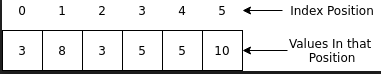
\includegraphics[scale=0.5]{arrays1.png}
	\caption{Image from Lecture}
\end{figure}

Imagine, if you will, having a bunch of variables of the same type under one name. This is essentially what an array is. So if you need to store a collection of integers, you can declare one array to store them instead of declaring a bunch of different variables. If you look at the table, the top row corresponds to the index position of the array. The index is simply where that particular piece of data is stored at in the array. Also note that we refer to these ``pieces of data`` as elements. For example, if we look at the table above, we can see that $8$ is an element of that array at index position $1$. \\

Notice that we start counting from $0$. The $0$th element is actually the first element in the array. Next, you can see all the boxes (aka the elements). Think of each box as a variable that you don`t have to name that stores a value. So in the image, we have an array of size $6$ that stores $6$ integers.\\

\subsection{Declaring/Initializing an Array}
We can declare an array just like we declare any other variable, in the form of
\begin{lstlisting}
int myArray[];
\end{lstlisting}

\section{Looping Over Arrays (Video Series Lecture 22 and 23)}
\section{2D Arrays (Video Series Lecture 24 and 25)}
\section{Sorting Arrays: Insertion Sort Algorithm (Video Series Lecture 26 and 27)}
\section{Gotchas with Arrays}



\end{document}